\chapter{Querying}

%\begin{itemize}
%\item Details of the problem statement
%\item Querying method without exploiting MEC (Depth first or breadth first search of dependent variables, ie ancestors) 
%\item Speed of this querying method. 
%\end{itemize}

\section{Outline of the Task}

%\null \quad \quad Given a Bayesian network $B$ and a query, our goal is to find a MEC equivalent graph $B'$ such that the number of nodes which must be computed is minimized for the same query over $B'$. By minimizing the number of nodes which must be computed, we can speed up the querying process to achieve faster inference. \newline


\null \quad \quad The first step toward our goal is to determine the set of random variables which must be involved in the computation to answer a given query over $G$. This will serve as a quantity we minimize in later chapters; the minimization will be to reduce the size of the set, meaning to find a Markov equivalent graph $G'$ to $G$ such that this number of vertices involved is minimized. \newline
\null \quad \quad Naturally, before we consider the minimization itself, we begin by identifying such a set of vertices. This chapter will focus on identifying this set of vertices which must be computed to answer a query, and given this, quantifying the computational cost of answering a query in general. 

\section{Structure of a Query}

\null \quad \quad An inference query is a question which asks the probability of an event given some observations. Queries can take advantage of multiple observations and have multiple targets. For example, one can ask for the probability that the random variable $X$ has takes on the value $x$ given that we have observed $Y = y$. Let $x$ be a value attained by the random variable $X$, and let $y$ be a value attained by the variable $Y$. This is written $p(X=x|Y=y)$. The general form of a query is as follows:

\begin{definition}[Query] Given a graph $G = (V,E)$ with $X_{1}, ...X_{m}, Y_{1}, ...Y_{n} \in V$, the general form of a query $q$ is $p(X_{1}, ..., X_{m} | Y_{1}, ... Y_{n})$, meaning the probability of variables $X_{1}, ..., X_{m}$ given that we have conditioned on observed values attained by variables $Y_{1}, ..., Y_{n}$. 
\end{definition}

\begin{remark}
Note that while a query on $G=(V,E)$ must have at least one target (otherwise there is nothing to compute), it does not necessarily need to include a condition. For example, $p(X=x)$ is a valid query for $X \in V$. 
\end{remark}

\begin{table}[h!]

  \begin{center}
  \scalebox{0.7}{ %----
    \begin{tabular}{  l | l | l | l  }
      \thead{Scenario} & \thead{Query} & \thead{Interpretation} & \thead{Example} \\
      \hline
      
       	\newline
 	\newline
      \makecell[l]{Query with a single \\ target and no \\ observations} &  \makecell[l]{$p(X=x)$} & \makecell[l]{Probability that $X=x$} & \makecell[l]{Probability that a patient \\ has lung cancer.} \\
      
 	\newline
 	\newline
      \makecell[l]{Query with a single \\ target, single \\ observation} &  \makecell[l]{$p(X=x|Z=z)$} & \makecell[l]{Probability that $X=x$ \\ given that we have \\ observed $Z=z$.} & \makecell[l]{Probability that a patient \\ has lung cancer given that \\ they are a tobacco smoker.} \\
 
      \newline
      \newline
      \makecell[l]{Query with multiple \\ targets, single \\ observation} &  \makecell[l]{$p(X=x,Y=y|Z=z)$} & \makecell[l]{Probability that $X=x$ and \\ $Y=y$ given that we have \\ observed $Z=z$.} & \makecell[l]{Probability that a patient \\ has lung cancer and high blood \\ pressure given that they are a \\ tobacco smoker.} \\
      
      \newline
      \newline
            \makecell[l]{Query with a single \\ target, multiple \\ observations} & \makecell[l]{$p(X=x|W=w,Z=z)$} & \makecell[l]{ Probability that $X=x$ \\ given that we have \\ observed $W=w$ and $Z=z$. } & \makecell[l]{Probability that a patient has \\ lung cancer given that they \\ are over 50 years of age and \\ a tobacco smoker} \\
            
     \newline
            \makecell[l]{Query with multiple \\ targets, multiple \\ observations} & \makecell[l]{$p(X=x, Y=y|W=w,Z=z)$} & \makecell[l]{ Probability that $X=x$\\ and $Y=y$  given \\ that we have observed \\ $W=w$ and $Z=z$. } & \makecell[l]{Probability that a patient has \\ lung cancer and high blood\\ pressure given that they \\ are over 50 years of age and \\ a tobacco smoker.} \\

    \end{tabular}
      } % ----
	\caption{Examples of possible queries which may be asked on a DAG $G$.}
  \end{center}
  \end{table}
  
  
\null \quad \quad Let $G$ be a DAG and $q$ a query. Define $\Delta(G, q)$ to be the set of vertices involved in the computation of $q$ on $G$. The goal of this chapter is to find this set, and in doing so, determine its size. In Chapter $5$, we will to present a method for finding $\argmin_{G' \in [G]} (|\Delta(G,q)|)$. We call this minimized graph $\Delta^{*}$.

\section{Vertices Required to Compute a Query}

\null \quad \quad In the following section, we determine which set of vertices a query $q$ on a DAG $G$ depends on, notated $\Delta(G,q)$. First we consider queries with single targets and single conditions, then move on to scenarios with multiple conditions, before finally generalizing to scenarios with multiple targets and conditions. We will see that the structure of the DAG (namely, position of targets in $G$ in relation to the position of conditions) plays a significant role in whether certain vertices must be involved in the computation of a query. \newline
\null \quad \quad Determining $\Delta(G,q)$ (and therefore $|\Delta(G,q)|$) for arbitrary $G$ and $q$ will later allow us to quantify the speedups gained by transforming the graph:  given a DAG $G$ and a Markov equivalent transformed DAG $G'$, we will compare $|\Delta(G,q)|$ to $|\Delta(G',q)|$. If $|\Delta(G',q)|$ is smaller, then one can conclude that the result of the transformation reduces the cost of answering the query. Then the question becomes whether the overhead of transformation is worth the earned speedup. \newline 
\null \quad \quad Once again, we will take advantage of the definition of conditional independence: $$P(A|B) = \frac{P(A,B)}{P(B)}.$$ 

\begin{lemma}
Computing a conditionless query $q = p(X_{0}, X_{1}, ..., X_{n})$ over a DAG $G$ depends on vertices $X_{0}, X_{1}, ..., X_{n}$ and all of their ancestors: $\alpha(X_{0}), \alpha(X_{1}), ..., \alpha(X_{n})$. 
\end{lemma}

\begin{proof}
Let $q = p(X_{0}, X_{1}, ..., X_{n})$ on a DAG $G$. Using the definition of a Bayesian network, we have that the joint probability distribution 
$$p(X_{0}, X_{1}, ... X_{n}) = \prod_{i=0}^{n} p(X_{i}|\prod\nolimits_{X_{i}}^{G}).$$ 
Therefore $q$ indeed depends on all ancestors of the targets. 
\end{proof}


%--------------------------------------threenode query example
\begin{example}\label{qe1}


 Let $q = p(X_{1} = x_{1})$ be a query on $G = (V,E)$ in Figure~\ref{fig:qe1}. The computation of $q$ is as follows:
 \begin{figure}[h!]
\centering
\begin{tikzpicture}
\Vertex[x=0, y=0, size=.5, color=white, label=$X_{1}$]{x1}
\Vertex[x = 2, y=0, size=.5, color=white, label=$X_{2}$]{x2}
\Vertex[x=4, y=0 ,size=.5,color=white, label=$X_{3}$]{x3} 
\Edge[Direct, distance=0.5](x3)(x2)
\Edge[Direct, distance=0.5](x2)(x1)
\Text[x = 2, y = -1]{$G$}
\end{tikzpicture}
\caption{}
\label{fig:qe1}
\end{figure}
 \begin{align*}
	p(X_{1} = x_{1}) & 	\ \ = \ \ \sum_{x_{2}} \sum_{x_{3}} p(X_{1}=x_{1}|X_{2}=x_{2}) \cdot p(X_{2}=x_{2}|X_{3}=x_{3}) \cdot p(X_{3}=x_{3}), \\
\end{align*}
and therefore requires considering the target vertex $X_{1}$ and its ancestors, namely $X_{2}$ and $X_{3}$.
\end{example}
%--------------------------------------\threenode query example


\begin{definition} \label{thm:querycostonetarget}
Let $q = p(X|Y)$ be a query on a DAG $G$. We refer to the cases that the computation of $q$ falls under as the following, depending on the position of $Y$ in $G$: 
\begin{itemize}
\item \textbf{Special case} If $X$ is conditionally independent of all ancestors of $Y$ given $Y$, then $q$ depends on $X$, $\alpha(X)\textbackslash \alpha(Y)$, and all vertices on a route from $X$ to $Y$ excluding $Y$ itself. 
\item \textbf{General case} Otherwise, in the case that $X$ is \textbf{not} independent of $\alpha(Y)$ given $Y$, $q$ depends on both $X$ and $Y$ in addition to the sets $\alpha(X)$ and $\alpha(Y)$. 
\end{itemize}
\end{definition}

\begin{remark}
The motivation for the contents of these sets is given via Theorem \ref{thm:querycost}.
\end{remark} 

\begin{remark}
Intuitively, one would assume that the General case also requires $\Delta(G,q)$ to contain all vertices on a route from $X$ to $Y$. This is only sometimes correct; we argue in Lemma~\ref{routeandancestors} that the inclusion of vertices along such a route is already covered by $\alpha(X) \cup \alpha(Y)$ when necessary, and is not included in $\alpha(X) \cup \alpha(Y)$ when $Z$ is not required in $\Delta(G,q)$.
\end{remark}


\begin{figure}[h!]
\begin{center}
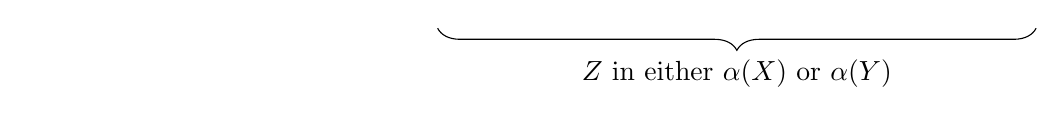
\begin{tikzpicture}
\Vertex[x = 0, y=3, size=.5, color=white, label=$X$]{x}
\Vertex[x = 0, y=1.5, size=.5, color=white, label=$Z$]{y}
\Vertex[x=0, y = 0, size=.5,color=white, label=$Y$]{z}
\Edge[Direct, distance=0.5](x)(y)
\Edge[Direct, distance=0.5](y)(z)
\Text[x=-.8 ,y=3]{$G_{1}$}

\Vertex[x = 3, y=3, size=.5, color=white, label=$X$]{x}
\Vertex[x = 3, y=1.5, size=.5, color=white, label=$Z$]{y}
\Vertex[x=3, y = 0, size=.5,color=white, label=$Y$]{z}
\Edge[Direct, distance=0.5](y)(x)
\Edge[Direct, distance=0.5](y)(z)
\Text[x=2.2 ,y=3]{$G_{2}$}

\Vertex[x = 6, y=3, size=.5, color=white, label=$X$]{x}
\Vertex[x = 6, y=1.5, size=.5, color=white, label=$Z$]{y}
\Vertex[x=6, y = 0, size=.5,color=white, label=$Y$]{z}
\Edge[Direct, distance=0.5](z)(y)
\Edge[Direct, distance=0.5](y)(x)
\Text[x=5.2 ,y=3]{$G_{3}$}

\Vertex[x = 10, y=3, size=.5, color=white, label=$X$]{x}
\Vertex[x = 10, y=1.5, size=.5, color=white, label=$Z$]{y}
\Vertex[x=10, y = 0, size=.5,color=white, label=$Y$]{z}
\Edge[Direct, distance=0.5](z)(y)
\Edge[Direct, distance=0.5](x)(y)
\Text[x=9.2 ,y=3]{$G_{4}$}

\draw [decorate,decoration={brace,amplitude=8pt,mirror,raise=-5ex}]
  (-.8,-1.3) -- (6.8,-1.3) node[midway,yshift=.5em]{$Z$ in either $\alpha(X)$ or $\alpha(Y)$};
\draw [decorate,decoration={brace,amplitude=8pt,mirror,raise=-5ex}]
  (9,-1.3) -- (11,-1.3) node[midway,yshift=.5em]{$Z$ not in $\alpha(X)$ nor $\alpha(Y)$};
\end{tikzpicture}
\end{center}
\caption{}
\label{ancestorinclusion}
\end{figure}


\begin{lemma} \label{routeandancestors}
Let $X$ and $Y$ be two vertices in a DAG $G$. Let $Z$ be the vertex on a route between $X$ and $Y$. Then $Z$ is either included in the set $\alpha(X) \cup \alpha(Y)$, or is not required in $\Delta(G,q)$. 
\end{lemma}

\begin{proof}
To demonstrate this, consider all possible arrangements of three such connected vertices $X$, $Y$, and $Z$, as shown in Figure~\ref{ancestorinclusion}. In the first three graphs, $G_{1}, G_{2}$ and $G_{3}$, $Z$ is clearly an ancestor of either $X$, $Y$, or both simultaneously. Therefore $Z$ is already included through the inclusion of the sets $\alpha(X)$ and $\alpha(Y)$ in the cases of $G_{1}, G_{2}$, and $G_{3}$. Then, we consider the fourth arrangement, $G_{4}$. We will show that in this scenario, $Z$ is not required to compute either $p(X|Y)$ or $p(Y|X)$. Without loss of generality, we show this for $p(X|Y)$. We can express it as the following: \newline
$$p(X|Y) = \frac{\sum_{Z} p(Z|X,Y)\cdot p(X)\cdot p(Y)}{p(Y)}.$$ Here, both $p(X)$ and $p(Y)$ are conditionally independent of $Z$, since here, $Z$ is not a parent of either of them. Therefore, we can pull both $p(X)$ and $p(Y)$ out of the sum $\sum_{Z}p(Z|X,Y)\cdot p(X) \cdot p(Y)$. This gives us 
$$\sum_{Z} (p(Z|X,Y)\cdot p(X) \cdot p(Y)) = p(X) \cdot p(Y) \cdot \sum_{Z} p(Z|X,Y).$$
Noticing that $\sum_{Z}p(Z|X,Y)$ is a probability density, it must equal $1$. Therefore the above becomes 
$$p(X) \cdot p(Y) \cdot 1 = p(X) p(Y)$$
which does not depend on $Z$. We conclude that $Z$ is not necessary for the computation of $p(X|Y)$, and without loss of generality, $p(Y|X)$. \newline
\null \quad \quad Furthermore, we affirm that $Z$ is necessary in the cases of $G_{1}, G_{2},$ and $G_{3}$ by showing that the computations applied to $G_{4}$ cannot be applied to these cases. This can be seen by realizing that in the first three graphs, at least one of the vertices $X$ and $Y$ depends on $Z$, and therefore $p(X)$ and $p(Y)$ cannot be pulled out of the sum, since they are not conditionally independent of $Z$. The results is that $Z$ must remain in $\Delta(G,q)$ in these cases. 
\end{proof}

%\begin{corollary} 
%Lemma~\ref{routeandancestors} holds for a set $\mathcal{Z}$ such that each $Z_{i} \in \mathcal{Z}$ is on the route between $X$ and $Y$, but $X$ and $Y$ do not depend on any $Z_{i}$. 
%\end{corollary}

%\begin{proof}
%This can be seen using fact that $G$ is acyclic: if $G$ is acyclic, and $Z_{1}, Z_{2},...Z_{n}$ are on a route from $X$ to $Y$, then without loss of generality, each element $Z_{i} \in \mathcal{Z} =\{Z_{0},Z_{1},...,Z_{i} \}$ is either (1), in $\alpha(X) \cup \alpha(Y)$, or (2), $p(X)$ and $p(Y)$ are conditionally independent of from $Z_{i}$. If this were not the case, we would be able to find a cycle from some $Z_{i}$ back to $X$ or $Y$ which are themselves ancestors of $Z_{i}$.
%\end{proof}

% To see this, we derive a contradiction: \newline 
%\null \quad \quad Suppose $Z_{i} \in \mathcal{Z}$ is, without loss of generality, an ancestor of $X$. The
%\null \quad \quad Trivially, if we suppose that $Z_{i} \in \mathcal{Z}$ is \textbf{not} an ancestor of $X$ or $Y$, but $p(X)$ and $p(Y)$ are not conditionally independent of it, we derive a contradiction since $p(X)$ and $p(Y)$ must then dependent on it, and therefore be descendants of it. Thus, $Z_{i}$ must either be an ancestor, or $p(X)$ and $p(Y)$ msut be conditionally independent from it. 
%\end{proof}

\begin{lemma}\label{lemma:alternativecases}
 The conditions for the cases in Definition~\ref{thm:querycostonetarget} can be rephrased as follows: 
\begin{itemize}
\item The condition $Y$ is in the \textbf{special case} if, when $Y$ is removed from $G$, the resulting graph $G'$ consists of at least two disconnected subgraphs $G'_{1}$ and $G'_{2}$ such that $X \in G'_{1}$ and all vertices in $\alpha(Y) \in G'_{2}$. That is, removing $Y$ disconnects $\alpha(Y)$ from $X$.
\item The condition $Y$ is in the \textbf{general case} otherwise. That is, whenever the removal of $Y$ does not result in a disconnected graph such that $X$ and all vertices in $\alpha(Y)$ are in separate subgraphs. 
\end{itemize}
\end{lemma}

\begin{proof}
We prove this using the definition of conditional independence. Without loss of generality, assume that the graph contains exactly three vertices $X$, $Y$, and $Z$. If $Y$ is in the special case, where $X$ and $Z$ are conditionally independent given $Y$, then $p(X|Z,Y) = p(X|Y)$. Then, using this conditional independence the probability distribution can be dissected as follows:
\begin{align*}
 p(X,Y,Z)& \ \ = \ \ \prod_{V= X,Y,Z} p(V| \prod\nolimits_{V}^{G}) \\[1em]
& \ \ = \ \ p(X|\prod\nolimits_{X}^{G} \textbackslash Z) \cdot p(Z|\prod\nolimits_{Y}^{G} \textbackslash X) \cdot p(Y|\prod\nolimits_{Y}^{G}).
\end{align*}
Then, $X$ and $Z$ are in separate components after the removal of $Y$, and therefore are disconnected. \newline
\null \quad \quad In contrast, if $Y$ is in the general case, then $X$ and $Z$ are not conditionally independent given $Y$, and therefore the probability distribution cannot be separated into two disjoint components as above. This is because there is a path from $Z$ to $X$ after removing $Y$. We conclude that $X$ and $Z$ are still connected. \newline
\null \quad \quad Since this was done without loss of generality, the above proof holds for sets of vertices $\mathcal{X} = \{X_{1}, ... X_{m}\}$ (and likewise for $Y$ and $Z$.)
\end{proof}

%%%%%%%%%%%%%%%%%%%%%%%%%%%%%%%%%%%%

%----------------------Example of general VS special case
 \begin{figure}[h!]
\centering
\begin{center}
\begin{tikzpicture}
\Vertex[x=-1.3=,y=2, size=.5, color=white, label=$Z$]{Z}
\Vertex[x=1.3,y=2, size=.5, color=white, label=$W$]{W}
\Vertex[x=0,y=.7 ,size=.5, color=white, label=$Y$]{Y} 
\Vertex[x=0, y=-.7, size=.5, color=white, label=$X$]{X}

\Edge[Direct, distance=0.5](Z)(X)
\Edge[Direct, distance=0.5](Y)(X)
\Edge[Direct, distance=0.5](Z)(Y)
\Edge[Direct, distance=0.5](W)(Y)


\Vertex[x=4.7=,y=2, size=.5, color=white, label=$Z$]{Z}
\Vertex[x=7.3,y=2, size=.5, color=white, label=$W$]{W}
\Vertex[x=6,y=.7 ,size=.5, color=white, label=$Y$]{Y} 
\Vertex[x=6, y=-.7, size=.5, color=white, label=$X$]{X}

\Edge[Direct, distance=0.5](Y)(X)
\Edge[Direct, distance=0.5](Z)(Y)
\Edge[Direct, distance=0.5](W)(Y)

\Text[x =0, y= -1.5]{General case}
\Text[x=6,y=-1.5]{Special case}
\end{tikzpicture}
\end{center}
\caption{Example of one DAG in the general case and one in the special case.}
\label{fig:qe2}
\end{figure}

%----------------------\Example of general VS special case


\null \quad \quad When considering queries with more than one condition, one cannot classify the DAG $G$ as being either in the special case or general case, but rather, must classify each condition $Y_{j}$ into the cases. This is because a target $X$ might be independent of $\alpha(Y_{0})$ given a condition $Y_{0}$, but might still be dependent on $\alpha(Y_{1})$ given $Y_{1}$. Then, $Y_{0}$ would be in the special case, whereas $Y_{1}$ would be in the general case. As a result, the query would not depend on $Y_{0}$ and its ancestors, but would still depend on $Y_{1}$ and its ancestors. \newline
\null \quad \quad Furthermore, when considering multiple targets $X_{0}, X_{1}, ... X_{i}$, one must check whether a set of ancestors $\alpha(Y_{j})$ is independent of all vertices $X_{i}, i\in [0,m]$ given $Y_{j}$. Otherwise, if one of the targets was dependent on an ancestor of $Y_{j}$, the query $q$ would depend on that ancestor. From this, we arrive at Theorem ~\ref{thm:querycost}.

\begin{theorem} \label{thm:querycost}
Let $q = p(X_{0}, X_{1}, ..., X_{m} | Y_{0}, Y_{1}, ..., Y_{n})$ be a query on a DAG $G$. Then the computation of $q$ requires the following sets of vertices depending on the structure of $G$:
\begin{enumerate}
\item $q$ always depends on all $X_{i}$ and $\alpha(X_{i})\textbackslash \alpha(Y_{j})$ , 
\item For each $Y_{j}, j\in[0,n]$ in the special case, $q$ depends on all vertices along a route from each vertex $X_{i}, i\in [0,m]$ to $Y_{j}$, not including $Y_{j}$ itself, 
\item For each $Y_{j}, j\in[0,n]$ in the general case, $q$ depends on vertices $Y_{j}$ and $\alpha(Y_{j})$.
\end{enumerate}

Therefore, if $Y_{j}$ is in the special case, $q$ does not depend on $Y_{j}$ nor $\alpha(Y_{j})$. 
\end{theorem}

\begin{proof}
Without loss of generality, suppose we have three vertices $X$, $Y$, and $Z$. Then, let $q = p(X|Y)$ be a query asked on a DAG $G$. Using the definition of a Bayesian network, we have the following joint probability distribution in the general case:
$$p(X, Y) =  p(X|\prod\nolimits_{X}^{G}) \cdot p(Y|\prod\nolimits_{Y}^{G}).$$ \newline
\null \quad \quad Therefore $q$ indeed depends on all ancestors of target $X$ and the condition $Y$. As argued in~\cref{routeandancestors}, if a vertex $Z$ on the route between $X$ and each $Y$ is required to compute $q$, it is already included in the sets $\alpha(X)$ and $\alpha(Y)$: this is because a vertex $Z$ on such a route is either representable in terms of other vertices in the ancestor sets, or is already included in them. \newline
\null \quad \quad Next, we show that vertex $Y$ in the Special case can be excluded from $\Delta(G,q)$ in addition to the ancestors $\alpha(Y)$. Suppose all ancestors of $Y$ are conditionally independent of $X$ given $Y$. Then, when we condition on $Y=y$, we are setting it to a specific value and effectively removing from the model; ancestors of $Y$ no longer play a role since we are not interested in how they affect a fixed value, and they do not affect any variable past $Y$ in the model.\newline 
\null \quad \quad Likewise, all other variables are conditioned on $Y$ itself, and therefore we do not need to compute how $Y$ is affected. Therefore, we need only to consider vertices on a route from $X$ to $Y$ (in order to determine how $Y=y$ affects the targets), but not $Y$ or $\alpha(Y)$. \newline
\null \quad \quad The above reasoning holds for sets of vertices $\mathcal{X} = \{X_{1}, ... , X_{m}\}$, $\mathcal{Y}$ and $\mathcal{Z}$.
\end{proof}

\begin{center}
\begin{figure}[h!]
\centering
\scalebox{.8}{
   \begin{tikzpicture}
	        \node at (-2.25cm,2cm) [rectangle,draw, minimum size=.8cm, minimum width = 3cm] (ancestors) {$$};
	        	        \Text[x=-2.25,y=2]{$Z_{0}, Z_{1}, ..., Z_{k}$}
	        \node at (0cm,0cm) [circle,draw, minimum size=.8cm, thick] (Yjs) {$$};
        		        \Text[x=0,y=0]{$Y_{j}$}
	        \node at (-4.5cm,0cm) [rectangle,draw, minimum size=.8cm, minimum width=3cm] (Xjs) {$$};
	                  \Text[x=-4.5,y=0]{$X_{1}, X_{2}, ..., X_{m}$}
	       \draw (ancestors) -- (Yjs);
	       \draw (Xjs) -- (Yjs);
	       \Text[x=-2.25,y=-1]{Special case}
	       
	       
	        \node at (8.25cm,2cm) [rectangle,draw, minimum size=.8cm, minimum width = 3cm] (ancestors) {$$};
	        	        \Text[x=8.25,y=2]{$Z_{0}, Z_{1}, ..., Z_{k}$}
	        \node at (10.5cm,0cm) [circle,draw, minimum size=.8cm, thick] (Yjs) {$$};
        		        \Text[x=10.5,y=0]{$Y_{j}$}
	        \node at (6cm,0cm) [rectangle,draw, minimum size=.8cm, minimum width=3cm] (Xjs) {$$};
	                  \Text[x=6,y=0]{$X_{1}, X_{2}, ..., X_{m}$}
	       \draw (ancestors) -- (Yjs);
	       \draw (Xjs) -- (ancestors);
	       \draw (Xjs) -- (Yjs);
	       
	      \Text[x=8.25,y=-1]{General case}
	       
    \end{tikzpicture}
}
    \caption{Graphical structure of the two cases: in the general case, $X_{i}$s are not conditionally independent from all elements $Z_{k} \in \alpha(Y_{j})$ given $Y_{j}$. In the special case, they are.}
    \label{fig:querycases}
\end{figure}
\end{center}


\begin{example} Here, we apply Theorem~\ref{thm:querycost} to determine the set of vertices a query $q$ over the DAG $G$ in Figure~\ref{fig:querydependentex} depends on. An explicit calculation to verify this is not given here; instead, we simply identify the set. Such calculations will take place in later examples. \newline


 \begin{figure}[h!]
\centering
\begin{center}
\begin{tikzpicture}
\Vertex[x=1.5, y=0, size=.5, color=white, label=$X$]{X}
\Vertex[x=0, y=1.5, size=.5, color=white, label=$Y_{0}$]{Y0}
\Vertex[x=3, y=1.5, size=.5,color=white, label=$Y_{1}$]{Y1} 
\Vertex[x=0, y=3.5, size=.5, color=white, label=$Z_{0}$]{Z0}
\Vertex[x=1.5, y=3.5, size=.5,color=white, label=$W_{0}$]{W0} 
\Vertex[x=3, y=3.5, size=.5, color=white, label=$W_{1}$]{W1}


\Edge[Direct, distance=0.5](Y0)(X)
\Edge[Direct, distance=0.5](Y1)(X)
\Edge[Direct, distance=0.5](W0)(Y1)
\Edge[Direct, distance=0.5](W1)(Y1)
\Edge[Direct, distance=0.5](Z0)(Y0)
\Edge[Direct, distance=0.5](W0)(X)

\Text[x = 1.5, y = -1]{$G$}
\end{tikzpicture}
\end{center}
\caption{}
\label{fig:querydependentex}
\end{figure}

Suppose $q = p(X|Y_{0},Y_{1})$. Then, for each of the conditions $Y_{0}$ and $Y_{1}$, we determine whether it is in the general case of the special case. Immediately, we know that the query depends on at least the target $X$ and the set $\alpha(X)$. 
\begin{itemize}
\item $Y_{0}$ has only one ancestor, namely $Z_{0}$. $Z_{0}$ is conditionally independent of $X$ given $Y_{0}$. Therefore, the condition $Y_{0}$ is in the special case. As a result, $q$ does not depend on $Y_{0}$ nor $Z_{0}$. 
\item $Y_{1}$ has two ancestors, namely $W_{0}$ and $W_{1}$. $X$ is not conditionally independent from $W_{0}$ given $Y_{1}$, since we can find a route to $W_{0}$ which does not pass through $Y_{1}$. Therefore, $Y_{1}$ is in the general case, and we conclude that the query still additionally depends on $W_{0}$, $W_{1}$ and $Y_{1}$
\end{itemize}
We conclude that $\Delta(G,q) = \{X, Y_{1}, W_{0}, W_{1}\}$.  
\end{example}


%-------------------------------------fournode query example

\null \quad \quad The following examples verify which vertices are in the set $\Delta(G,q)$ outlined in Theorem ~\ref{thm:querycost}. First we present several computations in the general case, then computations in the special case. Finally, we show how two different queries over the same DAG $G$ can fall into each case. 

\begin{example}\label{ex:qe2}

\textbf{General Case.} Let $q = p(X_{3} = x_{3}, X_{4} = x_{4})$ be a query on $G = (V,E)$ in Figure~\ref{fig:qe2}. The computation of $q$ is as follows.
 
 \begin{figure}[h!]
\centering
\begin{center}
\begin{tikzpicture}
\Vertex[x=0, y=1, size=.5, color=white, label=$X_1$]{x1}
\Vertex[x = 3.5, y=0, size=.5, color=white, label=$X_{4}$]{x2}
\Vertex[x=3.5, y=2 ,size=.5,color=white, label=$X_{3}$]{x3} 
\Vertex[x = 1.8, y=1, size=.5, color=white, label=$X_{2}$]{x4}

\Edge[Direct, distance=0.5](x1)(x4)
\Edge[Direct, distance=0.5](x4)(x3)
\Edge[Direct, distance=0.5](x4)(x2)

\Text[x = 1.8, y = -1]{$G$}
\end{tikzpicture}
\end{center}
\caption{}
\label{fig:qe2}
\end{figure}
 
\begin{align*}
 q 	& \ \ = \ \  p(X_{3} = x_{3}, X_{4} = x_{4}) \\[1em]
	& \ \ = \ \ \sum_{x_{2}} \sum_{x_{1}} p(X_{3}=x_{3},X_{4}=x_{4}|X_{2}=x_{2}) \\[1em] 
		& \quad \quad \cdot p(X_{2}=x_{2}|X_{1}=x_{1}) \cdot p(X_{1}=x_{1}) & (1)\\[1em] 
	& \ \ = \ \ \sum_{x_{2}} \sum_{x_{1}} p(X_{3}=x_{3}|X_{2}=x_{2})p(X_{4}=x_{4}|X_{2}=x_{2}) \\[1em] 
		& \quad \quad  \cdot p(X_{2}=x_{2}|X_{1}=x_{1}) \cdot p(X_{1}=x_{1}) & (2)\\[1em] 
	& \ \ = \ \ \sum_{x_{2}} \sum_{x_{1}} p(X_{3}=x_{3}|X_{2}=x_{2}) \cdot p(X_{4}=x_{4}|X_{2}=x_{2}) \\[1em]  
		& \quad \quad \cdot p(X_{1}=x_{1}, X_{2}=x_{2}) & (3)
\end{align*}

where equality (1) is by construction of the Bayesian network and equality (2) comes from the definition of conditional probability since $X_{3}$ and $X_{4}$ are conditionally independent. Equality (3) comes from the following application of conditional probability:
\begin{align*}
p(X_{2}=x_{2}| X_{1}=x_{1}) \cdot p(X_{1}=x_{1})	& \ \ = \ \  p(X_{1}=x_{1}, X_{2} = x_{2}). 
\end{align*}

The query $q$ depends on the targets $X_{4}$ and $X_{3}$ and their parents, $X_{2}$ and $X_{1}$. 

\end{example}





%--------------------------------------\fournode query example



%-------------------------------------Querycost Example
\begin{example}

\textbf{General case.} The following example follows similar structure to Example~\ref{ex:qe2} and uses real values for the conditional probabilities. Consider the graph $G=(V,E)$ from ~\ref{fig:costofquery}, where a vertex $V$ takes a binary value $v \in [0,1]$, and suppose we are given a query $q = p(Y=1|Z=1)$. \newline
\begin{figure}[h!]
\centering
\begin{center}
\begin{tikzpicture}
\Vertex[x=0, y=1, size=.5, color=white, label=$X$]{x1}
\Vertex[x = 3.5, y=0, size=.5, color=white, label=$U$]{x2}
\Vertex[x=3.5, y=2 ,size=.5,color=white, label=$W$]{x3} 
\Vertex[x = 1.8, y=1, size=.5, color=white, label=$Y$]{x4}
\Vertex[x = 5.3, y=2, size=.5, color=white, label=$Z$]{x6}

\Edge[Direct, distance=0.5](x1)(x4)
\Edge[Direct, distance=0.5](x4)(x3)
\Edge[Direct, distance=0.5](x4)(x2)
\Edge[Direct, distance=0.5](x3)(x6)

\Text[x = 2.65, y = -1]{$G$}

\end{tikzpicture}
\end{center}
\caption{}
\label{fig:costofquery}
\end{figure}
\null \quad \quad Let the conditional probabilities be given by

\begin{align*}
	& p(X = 1) = 0.2 			& \\
	& p(Y = 1 | X = 0) = 0.6		& p(Y = 1 | X = 1) = 0.4 \\ 
	& p(W = 1 | Y = 0) = 0.4		& p(W = 1 | Y = 1) = 0.3 \\
	& p(Z = 1 | W = 0) = 0.7		& p(Z = 1 | W = 1) = 0.3 \\ 
	& p(U = 1 | Y = 0) = 0.8		& p(U = 1 | Y = 1) = 0.4 \\
\end{align*}


Then, the joint probability is given by $$p(X,Y,W,U,Z) = p(X) \cdot p(Y|X) \cdot p(U|Y) \cdot p(W|Y) \cdot p(Z|W).$$ 
\null \quad \quad The aim of this example is to demonstrate that our query depends on the set of ancestors $\alpha(Y)$ and the vertices on route from $Z$ to $Y$, in this case, the route $Y \rightarrow W \rightarrow Z$. For this computation, we set $Z=1$, and recall that since we are in a binary setting, for a vertex $V$ we have $p(V=0) = 1 - p(V=1)$. Then, to determine $p(Y=1|Z=1)$, we first compute $p(Y=1)$:

\begin{align*}
	p(Y = 1) 	& \ \ = \ \ \sum_{X} p(Y = 0|x) \cdot p(x) \\ 
			& \ \ = \ \ 0.6 \cdot 0.8 + 0.4 \cdot 0.2 \\
			& \ \ = \ \ 0.48 + 0.08 \\
			& \ \ = \ \ 0.56 \\
	P(Y = 0)        & \ \ = \ \  1 - p(Y=1) = 0.44. \\
\end{align*}

By similar calculation and plugging in the values $p(Y=1)$ and $p(Y=0)$, we obtain that $p(W = 0) = \sum_{Y} p(W=0|Y)p(Y) \approx 0.65$ and $P(W = 1) \approx 0.34$. Likewise, we compute $p( Z = 1) \approx 0.56$ and $p(Z = 0) \approx 0,43$. \newline
\null \quad \quad From here, we determine how the observation $Z=1$ affects the likelihood of values of $W$ and consequently $Y$. Bayes' theorem allows us to do the calculation using quantities specified in the conditional probabilities:

$$p(W=1 | Z = 1) \ \ = \ \ \frac{p(Z=1|W=1)\cdot p(W=1)}{p(Z=1)} \ \ \approx \ \ \frac{0.3 \cdot 0.34}{0.56} \ \ \approx \ \ 0.18.$$

Subsequently $p(W = 0 | Z = 1) \approx 0.81$. Now that we see how $W$ is affected by the observation that $Z = 1$, we can move upward in the set of ancestors to determine which vertices $Y$ is affected by. Continuing with our condition that $Z=1$ and applying Bayes' theorem again,

\begin{align*}
	p(Y = 1 | W = 1)  \ \ = \ \ \frac{ p(W = 1 | Y = 1) \cdot p(Y = 1) }{p(W=1)} \ \ \approx \ \ \frac{0.18 \cdot 0.44}{0.18} \ \ \approx \ \ 0.48.
\end{align*}

Finally,

\begin{align*}
	p(Y = 1 | Z = 1) 	& \ \ = p(Y = 1|W = 0)\cdot p(W = 0) + p(Y=1|W=1)\cdot p(W=1) \\ 
			& \ \ \approx \ \ (0.59 \cdot 0.81)+(0.48 \cdot 0.18) \\
			& \ \ \approx \ \ 0.17.
\end{align*}

Thus, by tracing the effects of the observation $Z=1$ on a route to $Y=1$ (contained within $\alpha(Z)$) and using the ancestors $\alpha(Y)$, we have answered the query $q = p(Y = 1|Z = 1)$. Notice that this computation did not involve the vertex $U$, which is neither an ancestor of $Y$ nor along the route between $Y$ and $Z$. 
\end{example}

%-------------------------------------\Querycost Example

%-------------------------------------Special case1 Example

 \begin{figure}[h!]
\centering
\begin{tikzpicture}
\Vertex[x=0, y=0, size=.5, color=white, label=$X_{1}$]{x1}
\Vertex[x = 2, y=0, size=.5, color=white, label=$X_{2}$]{x2}
\Vertex[x=4, y=0 ,size=.5,color=white, label=$X_{3}$]{x3} 
\Vertex[x=6, y=0 ,size=.5,color=white, label=$X_{4}$]{x4} 
\Edge[Direct, distance=0.5](x4)(x3)
\Edge[Direct, distance=0.5](x3)(x2)
\Edge[Direct, distance=0.5](x2)(x1)
\Text[x = 3, y = -1]{$G$}
\end{tikzpicture}
\caption{}
\label{fig:specialcase1}
\end{figure}

\begin{example} \textbf{Special Case.}  Let $q = p(X_{4}=x_{4}|X_{2}=x_{2})$ be a query on $G$ in Figure~\ref{fig:specialcase1}. Then the query only involves vertices $X_{4}, X_{3}$, and $X_{2}$, so there is no need to consider vertex $X_{1}$. This is because $X_{4}$ is conditionally dependent of $\alpha(X_{2}) = X_{1}$. 


$$ p(X_{4}=x_{4}|X_{2}=x_{2}) = \sum_{x_{3}} p(X_{4}=x_{4}|X_{3}=x_{3}) \cdot p(X_{3}=x_{3}|X_{2}=x_{2}).$$

\end{example}

%-------------------------------------\Special case 1 Example


%-------------------------------------Special case 2 Example



\begin{figure}[h!]
\centering
\begin{tikzpicture}
\Vertex[size=.5, color=white, label=$X_{1}$]{x1}
\Vertex[x = 2, size=.5, color=white, label=$X_{2}$]{x2}
\Vertex[y = -1.5, x=1 ,size=.5,color=white, label=$X_{3}$]{x3}
\Edge[Direct, distance=0.5](x1)(x3)
\Edge[Direct, distance=0.5](x2)(x3)
\end{tikzpicture}
\caption{}
\label{fig:comp1}
\end{figure}

\begin{example} This example compares two queries over the same graph $G$ in Figure~\ref{fig:comp1}. Let $q_{1} = p(X_{2} = x_{2}|X_{3}=x_{3})$ and let $q_{2} = p(X_{3}=x_{3}|X_{2}=x_{2})$. \newline
\null \quad \quad Note that $X_{2}$ is an ancestor of $X_{3}$, and trivially $X_{2}$ is not conditionally independent from $X_{2}$. Therefore $q_{1}$ is in the general case of Theorem~\ref{thm:querycost}, since the target of $q_{1}$ (namely $X_{2}$) is not disjoint from the ancestors of the condition, $\alpha(X_{3})$. The computation of $q_{1}$ therefore requires the target $X_{2}$, the ancestors $\alpha(X_{2})$, the condition $X_{3}$, and $\alpha(X_{3})$. These sets together involve $X_{1}, X_{2}$, and $X_{3}$. This dependence is verified:

\begin{align*}
q_{1} & \ \ = \ \ p(X_{2}=x_{2}|X_{3}=x_{3}) \\[1.2em]
& \ \ = \ \ \frac{p(X_{2}=x_{2},X_{3}=x_{3})}{p(X_{3}=x_{3})} \\[1em]
& \ \ = \ \ \frac{ \sum_{x_{1}} p(X_{1}=x_{1}) \cdot p(X_{2}=x_{2}) \cdot p(X_{3}=x_{3}|X_{1}=x_{1},X_{2}=x_{2})} { \sum_{x_{1}} \sum_{x_{2}} p(X_{1}=x_{1}) \cdot p(X_{2} = x_{2}) \cdot p(X_{3}=x_{3}|X_{1}=x_{1},X_{2}=x_{2})}.
\end{align*}

\null \quad \quad Now we consider $q_{2}$. In this case, the conditional variable $X_{2}$ has no ancestors, and therefore we do not need to consider its distribution, since we are in the special case of Theorem~\ref{thm:querycost}. We show below that $q_{2}$ only relies only on $X_{3}$ and $X_{1}$. \newline

\begin{figure}[h!]
\centering
\begin{tikzpicture}
\Vertex[size=.5, color=white, label=$X_{1}$]{x1}
\Vertex[x = 2, size=.5, color=white, label=$X_{2}$]{x2}
\Vertex[y = -1.5, x=1 ,size=.5,color=white, label=$X_{3}$]{x3}
\Edge[Direct, distance=0.5](x1)(x3)
\Edge[Direct, distance=0.5](x2)(x3)

\Vertex[x=5, size=.5, color=white, label=$X_{1}$]{x11}
\Vertex[x = 7, size=.5, color=white, opacity={0.3}, label=$x_{2}$]{x21}
\Vertex[y = -1.5, x=6 ,size=.5,color=white, label=$X_{3}$]{x31}
\Edge[Direct, distance=0.5](x11)(x31)
\Edge[Direct, distance=0.5, color=gray, style={dashed}, opacity = {0.4}](x21)(x31)
\end{tikzpicture}
\caption{$X_{2}$ effectively removed from the model by conditioning $X_{2}=x_{2}$.}
\label{fig:comp1fade}
\end{figure}


\null \quad \quad Intuitively, setting $X_{2}=x_{2}$ effectively removes the variable from the model, since we are conditioning other variables on this observation. Once the other variables are adjusted, $X_{2}$ no longer plays a role since it already has an established value and does not have parents that must be considered. That is, we are setting $p(X_{3}=x_{3}|X_{1}=x_{1}) = p(X_{3}=x_{3}'|X_{1}=x_{1}', X_{2}=x_{2})$ for all $x_{1}', x_{2}'$. Thus:

\begin{align*}
q_{2} & \ \ = \ \ p(X_{3}=x_{3}|X_{2}=x_{2}) & \\[1em]
& \ \ = \ \ \frac{p(X_{3}=x_{3}, X_{2}=x_{2})}{p(X_{2}=x_{2})} \\[1em]
& \ \ = \ \ p(X_{3}=x_{3})  \\[1em]
& \ \ = \ \ \sum_{x_{1}} p(X_{3}=x_{3}|X_{1}=x_{1},X_{2}=x_{2}) \cdot p(X_{1}=x_{1}) \\[1em]
& \ \ = \ \ \sum_{x_{1}} p(X_{3}=x_{3}|X_{1}=x_{1}) \cdot p(X_{1}=x_{1}). 
\end{align*}

Therefore, $q_{2}$ relies only on $X_{3}$ and $X_{1}$ as described in the special case, whereas $q_{2}$ relies on $X_{2}$ as well, as described in the general case. 


\end{example}

\section{Arithmetic Complexity of Computing a Query}\label{section:complexityofaquery}

\null \quad \quad Once the set of vertices a query depends on ($\Delta(G,q)$) has been established, we can consider the arithmetic cost of the computations involved. The goal of this section is to determine the number of operations (+, $\cdot$) necessary to compute a query. We will calculate this arithmetic cost in terms of how it scales with the inputs of the query. \newline
\null \quad \quad Let $G = (V,E)$ be a DAG and $q$ a query. Let $\mathcal{X}, \mathcal{Y}, \mathcal{Z}, \subseteq V$, where targets $X_{i} \in \mathcal{X}$ and conditions $Y_{j}$ are in $\mathcal{Y}$. Let $\mathcal{Z}$ be the set of vertices which $q$ depends on, which are neither targets nor conditions: $\mathcal{Z} = \Delta(G,q) \textbackslash (\mathcal{X} \cup \mathcal{Y})$. Then, the form of $q$ is $q = p(\mathcal{X}|\mathcal{Y}) = p(X_{0},...X_{m}|Y_{0},...,Y_{n})$. In order to compute $q$, we must make the following calculations:
\begin{enumerate}
\item Compute the joint distribution $p(\mathcal{X},\mathcal{Y},\mathcal{Z})$, that is, of all variables in $\Delta(G,q)$.
\item Marginalize all $Z_{k} \in \mathcal{Z}$ out of $p(\mathcal{X},\mathcal{Y},\mathcal{Z})$. 
\item Compute the joint marginal distribution of $\mathcal{Y}$.
\item Condition the joint distribution $p(\mathcal{X},\mathcal{Y})$ to get $p(\mathcal{X}|\mathcal{Y})$.
\end{enumerate}

We will break the above operations into separate pieces and quantify the arithmetic cost of each piece in order to compute the total cost of answering $q$. We will present a general argument for the cost of each, and then contextualize it for binary variables. In this section, many computations will make use of the fact that in a binary setting, the sum over the possible assignments of values in a set $\mathcal{A}$ requires adding $2^{|\mathcal{A}|}$-many values. \newline

\textbf{(1) Compute the joint distribution $p(\mathcal{X}, \mathcal{Y}, \mathcal{Z})$}
\vspace{-4mm}

\begin{myindentpar}{1.5em}
\null \quad \quad We begin by determining the cost of calculating the full joint distribution for all vertices in $\Delta(G,q)$, namely $p(\mathcal{X},\mathcal{Y},\mathcal{Z})$. Recall that the joint distribution factorizes as 
$$p(V_{0},V_{1},...V_{|V|-1}) = \prod_{i \in |V|-1} p(V_{i}|\prod\nolimits_{G}^{V_{i}})$$
 where again, the set $\prod\nolimits_{G}^{V_{i}}$ is the set of parents of vertex $V_{i}$. In a binary setting, the number of specifications used to describe the distribution of vertex $V_{i}$ is therefore $2^{|\prod\nolimits_{V_{i}}^{G}|}$. For example, a vertex $X$ with one parent $Y$ is specified by $p(X|Y=1)$ and $p(X|Y=0)$, two distributions.\newline
 \null \quad \quad Notice that the number of parents of a given vertex is not necessarily restricted. We will address this in Chapter 5 when we calculate the complexity of various algorithms. For now, however, we recognize that the number of parents of a vertex is bounded by the number of vertices in $G$, and therefore replace $|\prod\nolimits_{V_{i}}^{G}|$ with $|V|$. \newline
\null \quad \quad The product is over $(|\mathcal{X}| + |\mathcal{Y}| + |\mathcal{Z}|)$-many variables, or equivalently, $|\Delta(G,q)|$-many variables. Then, using the fact that multiplying $n$ values together requires $(n-1)$ operations, the result is a cost of $\mathcal{O}(|\mathcal{X}|+|\mathcal{Y}|+|\mathcal{Z}|)\cdot 2^{|V|}$. We can also bound this as $\mathcal{O}(|\mathcal{X}|+|\mathcal{Y}|+|\mathcal{Z}|)\cdot 2^{|\mathcal{X}|+|\mathcal{Y}|+|\mathcal{Z}|}$ or, to be more asymptotically descriptive, $\mathcal{O}(|V|)\cdot 2^{|V|}$.
\end{myindentpar} 

\textbf{(2) Marginalize $\mathcal{Z}$ out of the distribution to determine $p(\mathcal{X}, \mathcal{Y})$}
\vspace{-4mm}

\begin{myindentpar}{1.5em}
\null \quad \quad Next, we marginalize the elements $Z_{k} \in \mathcal{Z}$ out of the joint distribution $p(\mathcal{X},\mathcal{Y},\mathcal{Z})$ to determine $p(\mathcal{X},\mathcal{Y})$. The joint marginal distribution is given by 
$$p(\mathcal{X},\mathcal{Y}) = \sum_{\mathcal{Z}} p(\mathcal{X},\mathcal{Y}, \mathcal{Z}).$$

Then, since we must compute the marginal for every possible assignment of $\mathcal{X}$ and $\mathcal{Y}$, this requires $2^{|\mathcal{X}|+|\mathcal{Y}|}$-many sums. Each sum has $2^{|\mathcal{Z}|}$ summands, making the total number of operations in $\mathcal{O}(2^{|\mathcal{X}| + |\mathcal{Y}| + |\mathcal{Z}|})$.
\end{myindentpar}

\textbf{(3) Compute the joint marginal distribution of the conditionals $\mathcal{Y}$}
\vspace{-4mm}

\begin{myindentpar}{1.5em}
\null \quad \quad Next, we must compute the joint marginal distribution $p(\mathcal{Y}) = p(Y_{0},...,Y_{n})$ from $p(\mathcal{X},\mathcal{Y})$. To do this, we determine the cost of computing the marginal for a single condition $Y_{j}$ and then multiply it by the number of marginal distributions which must be computed -- one for each condition -- which is $|\mathcal{Y}|$. The joint marginal distribution $p(\mathcal{Y})$ is given by 
$$p(\mathcal{Y}) = \sum_{\mathcal{X}} p(\mathcal{X}, \mathcal{Y}).$$
Likewise, the marginal distribution for a single value $Y_{j} \in \mathcal{Y}$ is given by
$$p(Y_{j}) = \sum_{\mathcal{X}} \sum_{Y_{i} \neq Y_{j}} p(\mathcal{X}, Y_{i})$$
 Again, computing the sum of $n$ values requires $(n-1)$ operations. Then, the sum over $\mathcal{X}$ requires $(2^{|\mathcal{X}|}-1)$ operations. For the marginals of each condition $Y_{j}$ to be computed, we need to sum over the $2^{|\mathcal{Y}|}$-many possible conditions. Therefore, there is a total cost is $\mathcal{O}(2^{|\mathcal{X}| + |\mathcal{Y}|})$.
\end{myindentpar}

\newpage

\textbf{(4) Condition the joint distribution}
\vspace{-4mm}

\begin{myindentpar}{1.5em}
\null \quad \quad Finally, we must condition on elements in $\mathcal{Y}$. That is, we must find the specialized distribution $p(\mathcal{X}|\mathcal{Y})$ by conditioning $p(\mathcal{X}, \mathcal{Y})$ on $\mathcal{Y}$. Using the definition of the conditional, we have
$$p(\mathcal{X}|\mathcal{Y}) = \frac{p(\mathcal{X},\mathcal{Y})}{p(\mathcal{Y})},$$
where again, $p(\mathcal{Y})$ is the joint marginal of all $Y_{0}, Y_{1},...Y_{j} \in \mathcal{Y}$. We already have the numerator and the denominator from Steps $(2)$ and $(3)$ above respectively, meaning we simply have to perform the relevant divisions in this step. In the binary setting this amounts to $2^{(|\mathcal{X}| + |\mathcal{Y}|)}$ divisions. Then Step $(4)$ is also $\mathcal{O}(2^{|\mathcal{X}|+|\mathcal{Y}|})$.
\end{myindentpar}

\textbf{Total}
\vspace{-4mm}

\begin{myindentpar}{1.5em}
 \null \quad \quad In composite, the above pieces allow us to calculate $q$. The complexities of each component add up as shown in Figure \ref{fig:costtable}.
 \begin{center}
 \begin{table}[h!]
 \centering
 \begin{tabular}{r r}
 \   & $\mathcal{O}((|\mathcal{X}|+|\mathcal{Y}|+ |\mathcal{Z}|)\cdot 2^{|\mathcal{X}|+|\mathcal{Y}|+|\mathcal{Z}|})$ \\[1em]
$+$ & $\mathcal{O}(2^{(|\mathcal{X}|+|\mathcal{Y}| + |\mathcal{Z}|)})$ \\[1em]
$+$ & $\mathcal{O}(2^{(|\mathcal{X}| + |\mathcal{Y}|)})$ \\[1em]
$+$ & $\mathcal{O}(2^{|\mathcal{X}| + |\mathcal{Y}|})$ \\[1em]
 \hline \\[-1em]
$=$ & $\mathcal{O}(2^{|\mathcal{X}|+|\mathcal{Y}|+|\mathcal{Z}|})$ \\[1em]
 \end{tabular}
 \caption{}
 \label{fig:costtable}
 \end{table}
 \end{center}
\end{myindentpar}
We therefore see that reducing the size of $\mathcal{Z}$ has an exponential effect on the number or computations required to compute a query. 

\begin{theorem}
Let $G$ be a sparse DAG and let $q = p(\mathcal{X}|\mathcal{Y})$ with $\mathcal{X} = (X_{0},X_{1},...,X_{i})$, $\mathcal{Y} = (Y_{0},Y_{1},...Y_{j})$ and $(Z_{0},Z_{1},...,Z_{k}) = \mathcal{Z} = \Delta(G,q) \textbackslash (\mathcal{X} \cup \mathcal{Y})$. Then, if the size of $\mathcal{Z}$ is reduced by $n$, then the query cost is reduced by $2^{n}$.
\end{theorem}

\begin{proof}
This follows from the costs computed in Table$~\ref{fig:costtable}$. The complexity of answering $q$ is $\mathcal{O}(2^{|\mathcal{X}|+|\mathcal{Y}|+|\mathcal{Z}|})$. If we reduce $\mathcal{Z}$ by 1, we reduce the entire exponent by 1, and therefore, the entire cost is lowered by $2^{|\mathcal{X}|+|\mathcal{Y}|+|\mathcal{Z}|-1}$, meaning the final cost is half of the original cost. 
\end{proof}


\begin{remark}
Notice that reducing the size of $\mathcal{Z}$ (which is the desired result of edge reversals) only affects the complexity of the first two steps in the above querying process. 
\end{remark}

\begin{remark}
There are other ways to compute the marginals using the above steps. For example, if we had chosen to do the computations in the order (1), (3), (4), (2), would would arrive at the same marginal distribution. However, other orderings are more computationally expensive. Notice that if we did the steps in this order, the complexity of conditioning the joint distribution and computing the joint marginal distribution of the conditionals would each be increased from $\mathcal{O}(2^{|\mathcal{X}|+|\mathcal{Y}|})$ to $\mathcal{O}(2^{|\mathcal{X}|+|\mathcal{Y}|+|\mathcal{Z}|})$. It is therefore beneficial to begin the computation by computing the joint distribution, then marginalizing $\mathcal{Z}$ out before conditioning. 
\end{remark}


